\section[Model-Driven Engineering]{\glsdesc{mde}}
\label{sec:back:mde}

Abstraction, also called modelling, is the heart of all scientific discipline, including computer science~\cite{DBLP:journals/cacm/Kramer07}.
One will abstract a system, computer or not, a problem, or a solution to reason about it for a specific purpose.
Abstraction reduces the scope to relevant parts, removing the extra that complexify the understanding.
For example, a climatologist models all elements that impact the global climate (wind, ocean current, temperature, ...), ignoring local information, like the temperature under a forest, or global ones, like the solar system.
In contrast, astronomers model the solar system, ignoring all information regarding the Earth climate.

In computer science, different modelling formalisms have been proposed. 
We can cite the entity-relationship~\cite{DBLP:journals/tods/Chen76} that is used to describe the data model for relational databases.
In the web community, they use the ontology~\cite{DBLP:journals/ijmms/Gruber95} formalism to define the semantic web\footnote{The Semantic Web is defined as en extension of the Web to enable the processing by machines.}~\cite{berners2001semantic}.
The software engineering community applies the \gls{uml}~\cite{omg2017umlspec} to formalism software system structure or behaviour.

Extending this need for abstraction to all software engineering activities, practitioners have proposed the \gls{mde} methodology~\cite{DBLP:journals/computer/Schmidt06,DBLP:conf/ifm/Kent02}.
This methodology advocates the use of models, or abstractions, as primary software artefacts~\cite{DBLP:journals/software/WhittleHR14}.
The contributions proposed in this thesis are in line with this vision.
In the following sections, we give an overview of the \gls{mde} methodology and how we will use it.


\subsection{Principles and vision}

\paragraph{Global overview}    
Software systems tend to be more and more complex.
To tame this complexity~\cite{DBLP:conf/icse/FranceR07, DBLP:journals/computer/Schmidt06}, the \gls{mde} methodology suggests  to use \glspl{model} for all the steps of software development and maintenance~\cite{DBLP:journals/computer/Schmidt06, DBLP:series/synthesis/2017Brambilla, DBLP:conf/icse/HutchinsonRW11, DBLP:conf/uml/BakerLW05, DBLP:conf/icse/HutchinsonWRK11, DBLP:journals/software/AtkinsonK03a}: design, evolution, validation, etc.
The core idea of this approach is two reduce the gap between the problem and the solution space~\cite{DBLP:journals/computer/Schmidt06}.
Two main mechanisms have been defined: \gls{dsml} and model transformation.
The former is based on the separation of concern principle.
Each concern\footnote{The definition of concern is intentionally left undefined as it is domain-specific.} should be addressed with a specific language, which manipulates concepts, has a type system, and a semantics dedicated to this concern.
These languages allow to create and manipulate \glspl{model}, specific for a domain.
The latter enables engineers to generate automatically software artefacts, such as documentation, source code, or test cases.
Using these mechanisms, stakeholders can focus on their problem keeping in mind the big picture.
A well-known example is the Structured Query Language \linebreak (SQL)~\cite{SQL:Spec}
Using this language, engineers can query a relational database, the data model being the \gls{model}.
They don't have to consider indexes (hidden behind the concept of, for example, primary keys) or all the mechanisms to persist and retrieve data from the disk.

\paragraph{Advantages and disadvantages}
Defenders of the \gls{mde} approach mainly highlight the benefits of abstraction in software engineering\cite{DBLP:journals/computer/Schmidt06, DBLP:conf/ifm/Kent02, DBLP:conf/uml/BakerLW05}.
First, using the same \gls{model}, engineers can target different specific platforms.
For example, the ThingML~\cite{DBLP:conf/models/HarrandFMH16} language allow specifying the behaviour of the system through state machines.
The same ThingML code can be deployed on different platform such as Arduino, Raspberry Pi.
Second, thanks to the transformation engine, the productivity and efficiency of developers is improved.
Third, \glspl{model} allow engineers to implement verification and validation techniques, like model checking~\cite{DBLP:books/daglib/0020348}, which will enhance the software quality.
Finally, the \glspl{model} enable the separation of application and infrastructure code and the reusability of \glspl{model}.

However, the literature has also identified some drawbacks of the \gls{mde} approach~\cite{DBLP:conf/ifm/Kent02, DBLP:conf/uml/BakerLW05, DBLP:conf/models/WhittleHRBH13, DBLP:conf/icse/HutchinsonRW11}.
First, it requires a significant initial effort when the \gls{dsml} needs to be defined.
Second, current approaches do not allow the definition of very large \glspl{model}.
This drawback can be mitigated with new methods such as NeoEMF~\cite{DBLP:conf/ecmdafa/BenelallamGSTL14, DBLP:journals/scp/DanielSBTVGC17}, which enable the storage of large \glspl{model},  and Mogwaï~\cite{DBLP:conf/rcis/DanielSC16}, a query engine for large \glspl{model}.
Third, this approach suffers from poor tooling support, as they should be reimplemented for each \gls{model}.
As for the second drawback, recent contributions try to remove this limitation.
For example, we can cite the work of Bousse \etal \cite{DBLP:journals/jss/BousseLCWB18} that define a generic omniscient debugger\footnote{Debuggers, generally, allow engineers to execute step-by-step programs, that is, forward. An omniscient debugger is also able to go backwards: to navigate back in the previous states of a program~\cite{DBLP:journals/corr/cs-SE-0310016}.} for \gls{dsml}.
Third, introducing \gls{mde} in a software development team presents organisational challenges.
It changes the way developers interact and work together.
Finally, abstraction is a two edges sword.
Indeed, reasoning at an abstract level may be more complex as some prefer to work with concrete examples and based on simulation.

\paragraph{Fundamentals concepts}
\gls{mde} is based on three fundamentals concepts: \gls{metamodel}, \gls{model}, and model transformation.
In this thesis, we do not use any transformation technique.
In the next section, we thus detail the concept of \gls{metamodel} and \gls{model}.

\subsection[Metamodel, model]{\Gls{metamodel}, \gls{model}}

\begin{figure}
	\centering
	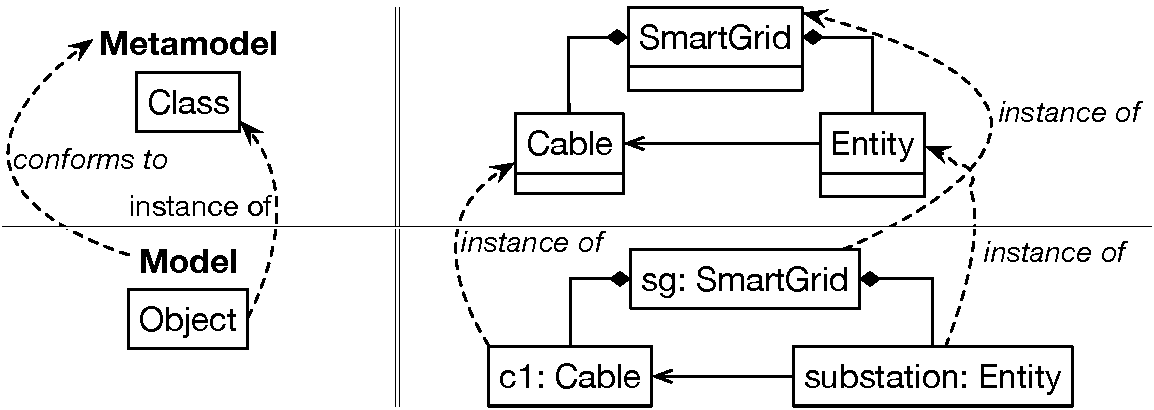
\includegraphics[width=0.8\linewidth]{img/chapt-background/mde/metavsmodel}
	\caption{Difference and relation between \gls{metamodel} and \gls{model}}
	\label{fig:background:mde:meta-model}
\end{figure}

\paragraph{\Gls{metamodel}}
\Glspl{metamodel} the different concepts in a domain and their relationships.
They represent the knowledge of a domain, for a specific purpose~\cite{DBLP:conf/iceccs/BezivinJT05}.
Also, they define the semantics rules and constraints to apply~\cite{DBLP:journals/computer/Schmidt06}.
They can be seen as \glspl{model} of \glspl{model}.
In the \gls{mde} community, they are generally defined using the class diagram of the \gls{uml} specification~\cite{omg2017umlspec}.
They, therefore, contain classes, named metaclass, and properties (attributes or references).
In the language engineering domain, \glspl{metamodel} are used to define the concepts that a language can manipulate (\cf \Cref{sec:back:sle}).
\gls{omg}\footnote{\url{https://www.omg.org/}} define a standard metamodeling architecture: \gls{mof}~\cite{MOF:Spec}.
It is set aside with \gls{ocl}~\cite{OCL:Spec}, the standard constraint language to define constraints that cannot be specified by a class diagram, and \gls{xmi}~\cite{XMI:Spec}, the standard data format to persist (meta)\glspl{model}. 

\paragraph{\Gls{model}}
\Glspl{model} capture some of the system characteristics into an abstraction that can be understood, manipulated, or processed by engineers or another system.
They are linked to their \glspl{metamodel} through the conformance relationship.
A \gls{model} is conformed to exactly one \gls{metamodel} if and only if it satisfies all the rules of the \gls{metamodel}.
That is, each element of a \gls{model} should instantiate at least one element of the \gls{metamodel} and respect all the semantics rules and constraints, that can be defined using \gls{ocl}.
Based on these models, stakeholders can apply verification and validation techniques, such as simulation and model checking, or model transformation.
France \etal have identified two classes of models~\cite{DBLP:conf/icse/FranceR07}: development and runtime models.
The former are abstraction above the code level.
It regroups requirements, architectural, or deployment models.
The latter abstract runtime behaviour or status of systems. 
%They are the basis of the \gls{m@rt} paradigm, which we detail in the next section.
They are the basis of the \gls{m@rt} paradigm, explained in~\Cref{sec:background:sas:m@rt}.
The models@run.time paradigm uses \glspl{metamodel} to define the domain concepts of a real system, together with its surrounding environment. 
Consequently, the runtime model depicts an abstract and yet rich representation of the system context that conforms to (is an instance of) its \gls{metamodel}.

%\subsection[Models@run.time]{\Gls{m@rt}}
%At its origins, \gls{mde} mainly addresses the challenges of designing, validating, and maintaining complex software systems.
%However, these systems were facing a new challenge: the uncertainty of the environment in which they are deployed.
%As we detail in \autoref{sec:back:adapt-syst}, systems have been improved to enable runtime adaptation.
%This process can only be done if the adaptation process has a deep understanding of the structure, the behaviour, and the environment of the system.
%This deep understanding can be provided by a proper abstraction of these runtime elements.
%Extending \gls{mde} principles and visions, the \gls{m@rt} paradigm spans the use of \glspl{model} from design time to runtime.
%The model, as an abstraction of a real system, can be used during runtime to reason about the state of the actual system. 
%A conceptual link between the model and the real system allows modifying the actual system through the model and vice versa.
%The models@run.time paradigm uses \glspl{metamodel} to define the domain concepts of a real system, together with its surrounding environment. 
%Consequently, the runtime model depicts an abstract and yet rich representation of the system context that conforms to (is an instance of) its \gls{metamodel}.

\subsection{Tooling}
Tooling is an essential aspect of every approach to be adopted.
Development platforms allow developers to create, manipulate, and persist (meta)\glspl{model} through high or low-level programming interfaces.
For example, a graphical language can be used for this purpose.
Additionally, these tools should embed transformation engines such as a code generator.

In the \gls{mde} community, the standard tool is the \gls{emf}~\cite{steinberg2008emf}.
It is the defacto baseline framework to build modelling tools within the Eclipse ecosystem.
It embeds its metamodelling  language, ECore~\cite{steinberg2008emf, ECore:website}.
ECore is thus the standard implementation of \gls{emof}~\cite{MOF:Spec}, a subset of \gls{mof} that corresponds to facilities found in object-oriented languages.
As written on the \gls{emf}-website\footnote{\url{https://www.eclipse.org/modeling/emf/}}, this modelling framework \textquote{provides tools and runtime support to produce a set of Java classes for the model, along with a set of adapter classes that enable viewing and command-based editing of the model, and a basic editor}. 

However, as highlighted by Fouquet \etal \cite{DBLP:journals/corr/FrancoisNMDBPJ14, DBLP:conf/models/FouquetNMDBPJ12}, models generated by EMF have some limitations, which prevent their use for the \gls{m@rt} paradigm.
The \gls{m@rt} can be used to implement an adaptive \gls{iot} systems\footnote{Definition of \gls{iot} by Gubbi \etal~\cite{DBLP:journals/fgcs/GubbiBMP13}: \textquote{Interconnection of sensing and actuating devices providing the ability to share information across platforms through a unified framework, developing a common operating picture for enabling innovative applications.}}.
These systems contain small devices, like micro-controllers, that have limited memory, disk space, and process capacity.
If one wants to deploy a model on it, thus it should have a low memory footprint, a low dependency size, a thread safety capacity, an efficient model (un)marshalling and cloning, a lazy loading mechanism, and compatibility with a standard design tool, here \gls{emf}.
However, the approaches at this time failed to tame the first four requirements.
They, therefore, define \gls{kmf}~\cite{DBLP:journals/corr/FrancoisNMDBPJ14, DBLP:conf/models/FouquetNMDBPJ12}, a modelling framework specific to the \gls{m@rt} paradigm.

Hartmann extended this work and created the \gls{gcm}\footnote{\url{https://github.com/datathings/greycat/tree/master/modeling}}.
Using this environment, a developer can create high-scalable models, designed for \gls{m@rt}\cite{DBLP:conf/seke/0001FNMKT14, DBLP:conf/models/Moawad0FNKT15}, with time as a first-class concept.
All metaclasses have a default time attribute to represent the lifetime of the model element that instantiates it.
The created models are object graphs stored on a temporal graph database, called GreyCat\footnote{\url{https://greycat.ai/}}~\cite{DBLP:journals/is/HartmannFMRT19, DBLP:phd/basesearch/Hartmann16}.
In addition to time, \glspl{metamodel} defined by \gls{gcm} can have an attribute with a value computed from a machine learning algorithm~\cite{DBLP:journals/sosym/0001MFT19}.
Based on the \gls{metamodel} definition, a Java and a Javascript \gls{api} are generated, to manipulate the model, \ie the temporal object graph.


\subsection{Concepts used in this thesis}
The \gls{m@rt} paradigm is a well-known approach to handle the challenges faced in \gls{adptSyst} development.
Plus, the \gls{gcm} has been designed to design a data model, with time as the first-class concept.
In this thesis, we will use this tool to define a \gls{metamodel} to abstract the knowledge of \glspl{adptSyst} (cf. \Cref{chapt:tkm}).

